
%% bare_conf.tex
%% V1.3
%% 2007/01/11
%% by Michael Shell
%% See:
%% http://www.michaelshell.org/
%% for current contact information.
%%
%% This is a skeleton file demonstrating the use of IEEEtran.cls
%% (requires IEEEtran.cls version 1.7 or later) with an IEEE conference paper.
%%
%% Support sites:
%% http://www.michaelshell.org/tex/ieeetran/
%% http://www.ctan.org/tex-archive/macros/latex/contrib/IEEEtran/
%% and
%% http://www.ieee.org/

%%*************************************************************************
%% Legal Notice:
%% This code is offered as-is without any warranty either expressed or
%% implied; without even the implied warranty of MERCHANTABILITY or
%% FITNESS FOR A PARTICULAR PURPOSE!
%% User assumes all risk.
%% In no event shall IEEE or any contributor to this code be liable for
%% any damages or losses, including, but not limited to, incidental,
%% consequential, or any other damages, resulting from the use or misuse
%% of any information contained here.
%%
%% All comments are the opinions of their respective authors and are not
%% necessarily endorsed by the IEEE.
%%
%% This work is distributed under the LaTeX Project Public License (LPPL)
%% ( http://www.latex-project.org/ ) version 1.3, and may be freely used,
%% distributed and modified. A copy of the LPPL, version 1.3, is included
%% in the base LaTeX documentation of all distributions of LaTeX released
%% 2003/12/01 or later.
%% Retain all contribution notices and credits.
%% ** Modified files should be clearly indicated as such, including  **
%% ** renaming them and changing author support contact information. **
%%
%% File list of work: IEEEtran.cls, IEEEtran_HOWTO.pdf, bare_adv.tex,
%%                    bare_conf.tex, bare_jrnl.tex, bare_jrnl_compsoc.tex
%%*************************************************************************

% *** Authors should verify (and, if needed, correct) their LaTeX system  ***
% *** with the testflow diagnostic prior to trusting their LaTeX platform ***
% *** with production work. IEEE's font choices can trigger bugs that do  ***
% *** not appear when using other class files.                            ***
% The testflow support page is at:
% http://www.michaelshell.org/tex/testflow/



% Note that the a4paper option is mainly intended so that authors in
% countries using A4 can easily print to A4 and see how their papers will
% look in print - the typesetting of the document will not typically be
% affected with changes in paper size (but the bottom and side margins will).
% Use the testflow package mentioned above to verify correct handling of
% both paper sizes by the user's LaTeX system.
%
% Also note that the "draftcls" or "draftclsnofoot", not "draft", option
% should be used if it is desired that the figures are to be displayed in
% draft mode.
%
\documentclass[10pt, conference, compsocconf]{IEEEtran}
% Add the compsocconf option for Computer Society conferences.
%
% If IEEEtran.cls has not been installed into the LaTeX system files,
% manually specify the path to it like:
% \documentclass[conference]{../sty/IEEEtran}





% Some very useful LaTeX packages include:
% (uncomment the ones you want to load)


% *** MISC UTILITY PACKAGES ***
%
%\usepackage{ifpdf}
% Heiko Oberdiek's ifpdf.sty is very useful if you need conditional
% compilation based on whether the output is pdf or dvi.
% usage:
% \ifpdf
%   % pdf code
% \else
%   % dvi code
% \fi
% The latest version of ifpdf.sty can be obtained from:
% http://www.ctan.org/tex-archive/macros/latex/contrib/oberdiek/
% Also, note that IEEEtran.cls V1.7 and later provides a builtin
% \ifCLASSINFOpdf conditional that works the same way.
% When switching from latex to pdflatex and vice-versa, the compiler may
% have to be run twice to clear warning/error messages.






% *** CITATION PACKAGES ***
%
%\usepackage{cite}
% cite.sty was written by Donald Arseneau
% V1.6 and later of IEEEtran pre-defines the format of the cite.sty package
% \cite{} output to follow that of IEEE. Loading the cite package will
% result in citation numbers being automatically sorted and properly
% "compressed/ranged". e.g., [1], [9], [2], [7], [5], [6] without using
% cite.sty will become [1], [2], [5]--[7], [9] using cite.sty. cite.sty's
% \cite will automatically add leading space, if needed. Use cite.sty's
% noadjust option (cite.sty V3.8 and later) if you want to turn this off.
% cite.sty is already installed on most LaTeX systems. Be sure and use
% version 4.0 (2003-05-27) and later if using hyperref.sty. cite.sty does
% not currently provide for hyperlinked citations.
% The latest version can be obtained at:
% http://www.ctan.org/tex-archive/macros/latex/contrib/cite/
% The documentation is contained in the cite.sty file itself.






% *** GRAPHICS RELATED PACKAGES ***
%
\ifCLASSINFOpdf
   \usepackage[pdftex]{graphicx}
  % declare the path(s) where your graphic files are
   \graphicspath{{../pdf/}{../jpeg/}}
  % and their extensions so you won't have to specify these with
  % every instance of \includegraphics
   \DeclareGraphicsExtensions{.pdf,.jpeg,.png}
\else
  % or other class option (dvipsone, dvipdf, if not using dvips). graphicx
  % will default to the driver specified in the system graphics.cfg if no
  % driver is specified.
   \usepackage[dvips]{graphicx}
  % declare the path(s) where your graphic files are
   \graphicspath{{../eps/}}
  % and their extensions so you won't have to specify these with
  % every instance of \includegraphics
   \DeclareGraphicsExtensions{.eps}
\fi
% graphicx was written by David Carlisle and Sebastian Rahtz. It is
% required if you want graphics, photos, etc. graphicx.sty is already
% installed on most LaTeX systems. The latest version and documentation can
% be obtained at:
% http://www.ctan.org/tex-archive/macros/latex/required/graphics/
% Another good source of documentation is "Using Imported Graphics in
% LaTeX2e" by Keith Reckdahl which can be found as epslatex.ps or
% epslatex.pdf at: http://www.ctan.org/tex-archive/info/
%
% latex, and pdflatex in dvi mode, support graphics in encapsulated
% postscript (.eps) format. pdflatex in pdf mode supports graphics
% in .pdf, .jpeg, .png and .mps (metapost) formats. Users should ensure
% that all non-photo figures use a vector format (.eps, .pdf, .mps) and
% not a bitmapped formats (.jpeg, .png). IEEE frowns on bitmapped formats
% which can result in "jaggedy"/blurry rendering of lines and letters as
% well as large increases in file sizes.
%
% You can find documentation about the pdfTeX application at:
% http://www.tug.org/applications/pdftex





% *** MATH PACKAGES ***
%
\usepackage[cmex10]{amsmath}
% A popular package from the American Mathematical Society that provides
% many useful and powerful commands for dealing with mathematics. If using
% it, be sure to load this package with the cmex10 option to ensure that
% only type 1 fonts will utilized at all point sizes. Without this option,
% it is possible that some math symbols, particularly those within
% footnotes, will be rendered in bitmap form which will result in a
% document that can not be IEEE Xplore compliant!
%
% Also, note that the amsmath package sets \interdisplaylinepenalty to 10000
% thus preventing page breaks from occurring within multiline equations. Use:
%\interdisplaylinepenalty=2500
% after loading amsmath to restore such page breaks as IEEEtran.cls normally
% does. amsmath.sty is already installed on most LaTeX systems. The latest
% version and documentation can be obtained at:
% http://www.ctan.org/tex-archive/macros/latex/required/amslatex/math/





% *** SPECIALIZED LIST PACKAGES ***
%
\usepackage{algorithm}
\usepackage{algorithmicx}
\usepackage{algpseudocode}
%\usepackage{algorithmic}
% algorithmic.sty was written by Peter Williams and Rogerio Brito.
% This package provides an algorithmic environment fo describing algorithms.
% You can use the algorithmic environment in-text or within a figure
% environment to provide for a floating algorithm. Do NOT use the algorithm
% floating environment provided by algorithm.sty (by the same authors) or
% algorithm2e.sty (by Christophe Fiorio) as IEEE does not use dedicated
% algorithm float types and packages that provide these will not provide
% correct IEEE style captions. The latest version and documentation of
% algorithmic.sty can be obtained at:
% http://www.ctan.org/tex-archive/macros/latex/contrib/algorithms/
% There is also a support site at:
% http://algorithms.berlios.de/index.html
% Also of interest may be the (relatively newer and more customizable)
% algorithmicx.sty package by Szasz Janos:
% http://www.ctan.org/tex-archive/macros/latex/contrib/algorithmicx/




% *** ALIGNMENT PACKAGES ***
%
%\usepackage{array}
% Frank Mittelbach's and David Carlisle's array.sty patches and improves
% the standard LaTeX2e array and tabular environments to provide better
% appearance and additional user controls. As the default LaTeX2e table
% generation code is lacking to the point of almost being broken with
% respect to the quality of the end results, all users are strongly
% advised to use an enhanced (at the very least that provided by array.sty)
% set of table tools. array.sty is already installed on most systems. The
% latest version and documentation can be obtained at:
% http://www.ctan.org/tex-archive/macros/latex/required/tools/


%\usepackage{mdwmath}
%\usepackage{mdwtab}
% Also highly recommended is Mark Wooding's extremely powerful MDW tools,
% especially mdwmath.sty and mdwtab.sty which are used to format equations
% and tables, respectively. The MDWtools set is already installed on most
% LaTeX systems. The lastest version and documentation is available at:
% http://www.ctan.org/tex-archive/macros/latex/contrib/mdwtools/


% IEEEtran contains the IEEEeqnarray family of commands that can be used to
% generate multiline equations as well as matrices, tables, etc., of high
% quality.


%\usepackage{eqparbox}
% Also of notable interest is Scott Pakin's eqparbox package for creating
% (automatically sized) equal width boxes - aka "natural width parboxes".
% Available at:
% http://www.ctan.org/tex-archive/macros/latex/contrib/eqparbox/





% *** SUBFIGURE PACKAGES ***
%\usepackage[tight,footnotesize]{subfigure}
% subfigure.sty was written by Steven Douglas Cochran. This package makes it
% easy to put subfigures in your figures. e.g., "Figure 1a and 1b". For IEEE
% work, it is a good idea to load it with the tight package option to reduce
% the amount of white space around the subfigures. subfigure.sty is already
% installed on most LaTeX systems. The latest version and documentation can
% be obtained at:
% http://www.ctan.org/tex-archive/obsolete/macros/latex/contrib/subfigure/
% subfigure.sty has been superceeded by subfig.sty.



%\usepackage[caption=false]{caption}
%\usepackage[font=footnotesize]{subfig}
% subfig.sty, also written by Steven Douglas Cochran, is the modern
% replacement for subfigure.sty. However, subfig.sty requires and
% automatically loads Axel Sommerfeldt's caption.sty which will override
% IEEEtran.cls handling of captions and this will result in nonIEEE style
% figure/table captions. To prevent this problem, be sure and preload
% caption.sty with its "caption=false" package option. This is will preserve
% IEEEtran.cls handing of captions. Version 1.3 (2005/06/28) and later
% (recommended due to many improvements over 1.2) of subfig.sty supports
% the caption=false option directly:
%\usepackage[caption=false,font=footnotesize]{subfig}
%
% The latest version and documentation can be obtained at:
% http://www.ctan.org/tex-archive/macros/latex/contrib/subfig/
% The latest version and documentation of caption.sty can be obtained at:
% http://www.ctan.org/tex-archive/macros/latex/contrib/caption/




% *** FLOAT PACKAGES ***
%
%\usepackage{fixltx2e}
% fixltx2e, the successor to the earlier fix2col.sty, was written by
% Frank Mittelbach and David Carlisle. This package corrects a few problems
% in the LaTeX2e kernel, the most notable of which is that in current
% LaTeX2e releases, the ordering of single and double column floats is not
% guaranteed to be preserved. Thus, an unpatched LaTeX2e can allow a
% single column figure to be placed prior to an earlier double column
% figure. The latest version and documentation can be found at:
% http://www.ctan.org/tex-archive/macros/latex/base/



%\usepackage{stfloats}
% stfloats.sty was written by Sigitas Tolusis. This package gives LaTeX2e
% the ability to do double column floats at the bottom of the page as well
% as the top. (e.g., "\begin{figure*}[!b]" is not normally possible in
% LaTeX2e). It also provides a command:
%\fnbelowfloat
% to enable the placement of footnotes below bottom floats (the standard
% LaTeX2e kernel puts them above bottom floats). This is an invasive package
% which rewrites many portions of the LaTeX2e float routines. It may not work
% with other packages that modify the LaTeX2e float routines. The latest
% version and documentation can be obtained at:
% http://www.ctan.org/tex-archive/macros/latex/contrib/sttools/
% Documentation is contained in the stfloats.sty comments as well as in the
% presfull.pdf file. Do not use the stfloats baselinefloat ability as IEEE
% does not allow \baselineskip to stretch. Authors submitting work to the
% IEEE should note that IEEE rarely uses double column equations and
% that authors should try to avoid such use. Do not be tempted to use the
% cuted.sty or midfloat.sty packages (also by Sigitas Tolusis) as IEEE does
% not format its papers in such ways.





% *** PDF, URL AND HYPERLINK PACKAGES ***
%
%\usepackage{url}
% url.sty was written by Donald Arseneau. It provides better support for
% handling and breaking URLs. url.sty is already installed on most LaTeX
% systems. The latest version can be obtained at:
% http://www.ctan.org/tex-archive/macros/latex/contrib/misc/
% Read the url.sty source comments for usage information. Basically,
% \url{my_url_here}.





% *** Do not adjust lengths that control margins, column widths, etc. ***
% *** Do not use packages that alter fonts (such as pslatex).         ***
% There should be no need to do such things with IEEEtran.cls V1.6 and later.
% (Unless specifically asked to do so by the journal or conference you plan
% to submit to, of course. )


% correct bad hyphenation here
\hyphenation{op-tical net-works semi-conduc-tor}


\begin{document}
%
% paper title
% can use linebreaks \\ within to get better formatting as desired
\title{MR. Prophet: Predicting the Performance of MapReduce Applications by Considering Phase Parallelism}
% author names and affiliations
% use a multiple column layout for up to two different
% affiliations
\author{\IEEEauthorblockN{Zhonghou Lv\textsuperscript{\dag},Hailong Sun\textsuperscript{\ddag},Xu Wang\textsuperscript{\dag},Xudong Liu\textsuperscript{\dag}}
\IEEEauthorblockA{School of Computer Science and Engineering\\
Beihang University\\
Beijing, China\\
\textsuperscript{\dag}\{lvzh, wangxu, liuxd\}@act.buaa.edu.cn, \textsuperscript{\ddag}sunhl@buaa.edu.cn}
}

% conference papers do not typically use \thanks and this command
% is locked out in conference mode. If really needed, such as for
% the acknowledgment of grants, issue a \IEEEoverridecommandlockouts
% after \documentclass

% for over three affiliations, or if they all won't fit within the width
% of the page, use this alternative format:
%
%\author{\IEEEauthorblockN{Michael Shell\IEEEauthorrefmark{1},
%Homer Simpson\IEEEauthorrefmark{2},
%James Kirk\IEEEauthorrefmark{3},
%Montgomery Scott\IEEEauthorrefmark{3} and
%Eldon Tyrell\IEEEauthorrefmark{4}}
%\IEEEauthorblockA{\IEEEauthorrefmark{1}School of Electrical and Computer Engineering\\
%Georgia Institute of Technology,
%Atlanta, Georgia 30332--0250\\ Email: see http://www.michaelshell.org/contact.html}
%\IEEEauthorblockA{\IEEEauthorrefmark{2}Twentieth Century Fox, Springfield, USA\\
%Email: homer@thesimpsons.com}
%\IEEEauthorblockA{\IEEEauthorrefmark{3}Starfleet Academy, San Francisco, California 96678-2391\\
%Telephone: (800) 555--1212, Fax: (888) 555--1212}
%\IEEEauthorblockA{\IEEEauthorrefmark{4}Tyrell Inc., 123 Replicant Street, Los Angeles, California 90210--4321}}




% use for special paper notices
%\IEEEspecialpapernotice{(Invited Paper)}




% make the title area
\maketitle
\begin{abstract}
MapReduce has been proved to be a successful programming model for big data processing. An accurate performance model has significant implication for optimizing the performance of MapReduce applications, which highly relies on the accurate anatomy of the execution process of a MapReduce application.
To speedup the processing of a MapReduce job, parallelism between multiple phases inside the task is widely employed in Hadoop and this parallelism is closely related to a set of configuration parameters at the same time.
Surprisingly we find that existing works on the MapReduce performance model scarcely consider the multi-phase parallelism, and most of efforts simply divide the task into a sequential flow, such as read, map, spill and merge inside the map task.
In this work, we propose a performance model for MapReduce applications, MR. Prophet, by fully incorporating the multi-phase parallelism inside the task into the model.
We also design and implement a lightweight performance instrumentation tool, LTrace, to collect some application and system specific statistical data so as to instantiate the model for an application.
Finally, we have conducted a set of experimental evaluation of our model with HiBench workload.
The results illustrate that MR. Prophet can achieve very high prediction accuracy and greatly outperforms the comparing model, for example, our model can achieve above 94\% accuracy for WordCount, TeraSort and PageRank jobs.
\end{abstract}


\begin{IEEEkeywords}
MapReduce; performance model; parallelism;
\end{IEEEkeywords}


% For peer review papers, you can put extra information on the cover
% page as needed:
% \ifCLASSOPTIONpeerreview
% \begin{center} \bfseries EDICS Category: 3-BBND \end{center}
% \fi
%
% For peerreview papers, this IEEEtran command inserts a page break and
% creates the second title. It will be ignored for other modes.
\IEEEpeerreviewmaketitle


\section{Introduction}
In recent years, with the rapid development of e-commerce, search engines, social networks and mobile internet,
the challenge of data processing has been growing rapidly due to the fast-growing volumes of data.
MapReduce~\cite{Dean2004MapReduce} is one of the most popular and efficient big data computing framework.
Hadoop~\cite{White2010Hadoop} is the most frequently-used open source implementation of MapReduce.
Programmers, researchers and even some computer science beginners can deal with big data processing jobs, such as log analysis, index building and data mining, on the platform of hadoop.

The performance prediction of MapReduce jobs can predict the jobs' execution cost, which has more and more utility value. For example, it can be applied to optimize the configuration parameters of MapReduce jobs to speed up the jobs' execution~\cite{Herodotou2011Profiling, Shi2014MRTuner, Li2014MRONLINE}, to dynamically adjust the number of cluster nodes for improving the cluster's resource utilization, and to select or implement the effective scheduling strategy. However, it is full of challenges to accurately forecast the execution cost of the MapReduce job. The high-precision performance prediction needs not only to forecast the execution cost of each individual phase, but it also is essential to predict the overlap time between multiple parallel phases. What is more, the MapReduce job's execution is affected by a number of factors, such as configuration parameters, input data and the user-defined programs. As a consequence, It has certain difficulty to accurately predict each individual phase's cost and  the overlap time between multiple parallel phases.

Nowadays, there are some related research~\cite{Herodotou2011Profiling, Shi2014MRTuner, Herodotou2011Hadoop} on the prediction of MapReduce job's execution time, which can be applied to optimize the configuration parameters ~\cite{Herodotou2011No}.  The construction of job's performance model is one of the most effective methods to forecast the execution time of MapReduce jobs. However, there are some deficiencies in the existing performance models. The present models are constructed to predict the executive cost of each individual phase of MapReduce, and the simple addition of each phase's cost is the prediction of the execution time. As a matter of fact, the executing procedure of a MapReduce job in Hadoop system is complicated, which is not computed step by step purely. For example, multi-threading technology leads to the parallel execution between multiple individual phases.

 To construct an accurate performance model for the MapReduce jobs, it is necessary to confirm whether the parallelism exists between multiple phases, and to measure the job's execution time in the presence of parallelism. We have analyzed the practical execution process of Hadoop MapReduce through reading its source code. As a result, we find that some fine-grained phases' execution parallels with others'. Furthermore, we have conducted a thorough analysis of the associated factors that affect the execution time of each fine-grained phase and the overlap time between multiple phases.

In addition, we need an extra lightweight monitoring and analysis tool to obtain the execution statistical data of MapReduce Jobs, and these statistics contain the statistical information about the dataflow and execution time of each fine-grained phase. The recent related works use the third-party profilers to capture the executive statistics, and this profiler increases the overhead by 5\%-30\%, which negatively affects the execution performance of the running MapReduce Jobs and consequently brings errors to the accuracy of statistics. To relieve the negative impact of the profiler's heavy overhead, we design a lightweight approach, which is based on the log printing system, to collect the statistics. The row data of the running jobs' execution information is printed to the log files through the log message firstly, and then the statistics are obtained off-line through the extraction of the log files. This approach separates the statistics collection into two phases, which minimize the negative impact of the profiler's overhead.

This paper introduces how to predict the execution time through the construction of the MapReduce performance model, the main contributions of this paper are as follows:
\begin{enumerate}
    \item  we construct a MapReduce performance model MR. Prophet, which can predict the execution time of a MapReduce job with high accuracy.
    \item  we design a lightweight log-based approach to capture the execution statistics of MapReduce jobs.
    \item  we have conducted extensive experiments with HiBench, and verified the accuracy of Mr. Prophet through the comparison with the related work.
\end{enumerate}

The rest of this paper is organized as follows. Section 2 presents a fine anatomy of the processing of MapReduce jobs. Section 3 introduces the design and implementation of the lightweight profiler, LTrace. Section 4 describes a new Hadoop MapReduce's performance model. Section 5 presents the evaluation results with HiBench workload. And Section 6 introduces some related work, finally Section 7 concludes this paper.


\section{Anatomy of MapReduce Job Execution}
This section introduces the executing procedure of running a MapReduce job in Hadoop.
\begin{figure}[htbp]
%\begin{figure}[!t]
\centering
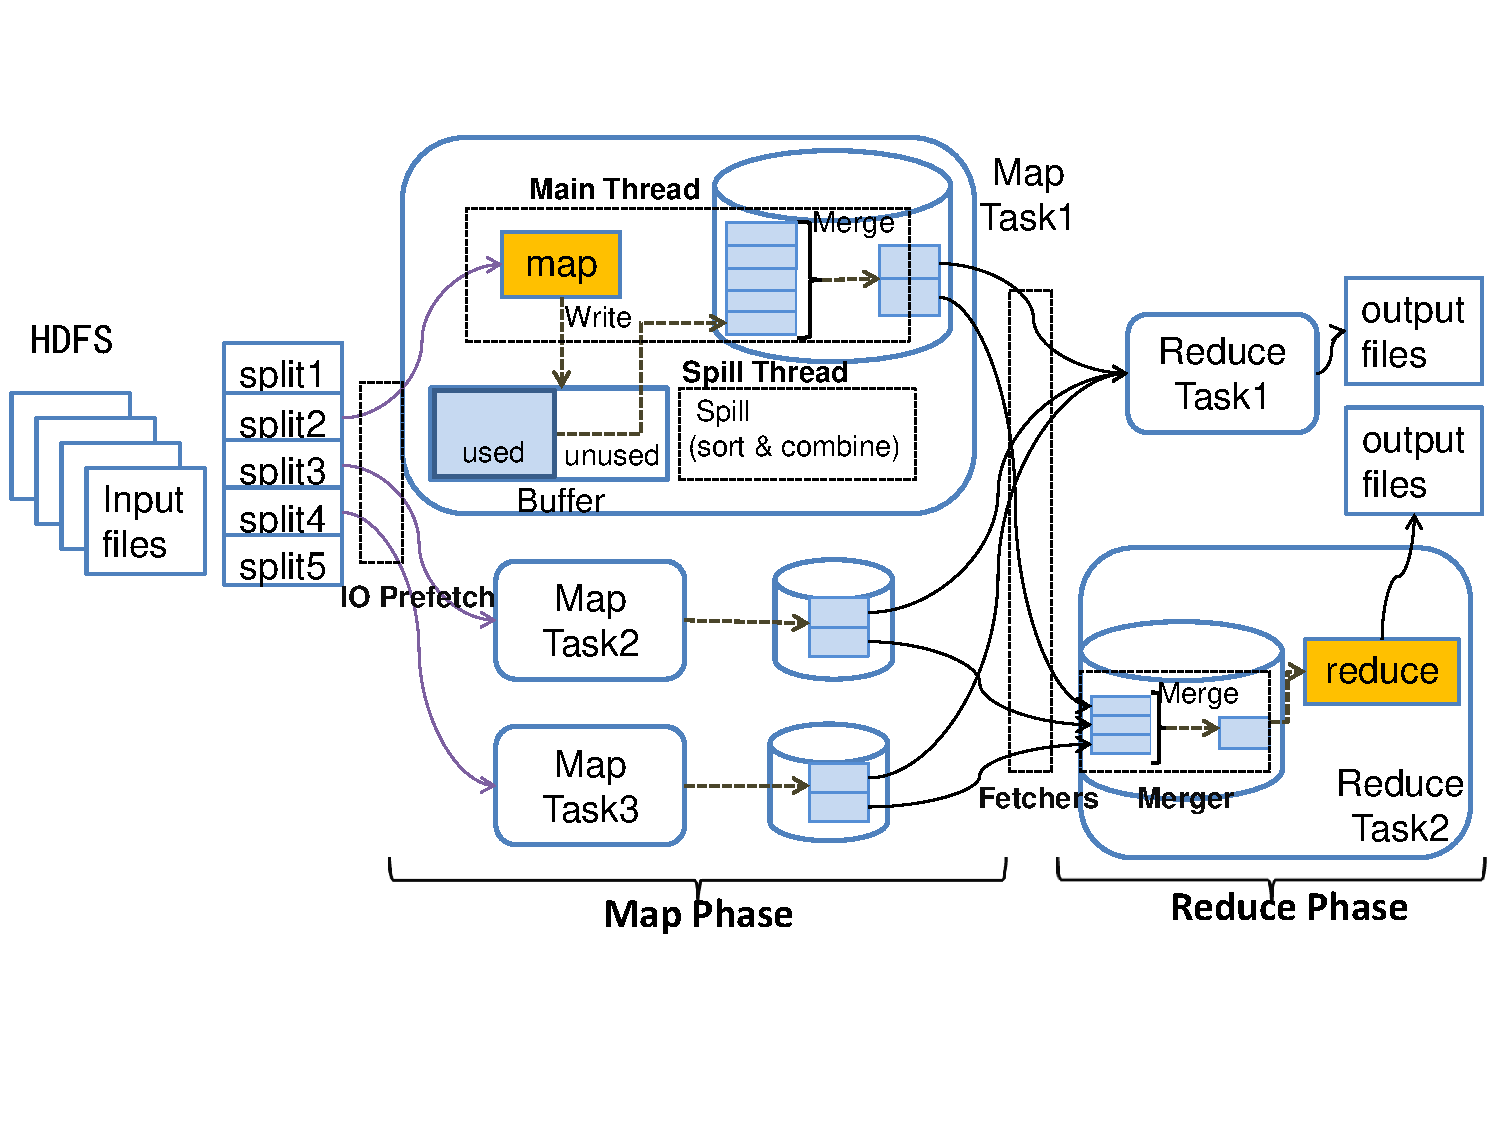
\includegraphics[height=5.25cm, width=8.65cm]{Job}
\caption{The execution procedure of map and reduce tasks}
\label{fig:mrprocedure}
\end{figure}

\noindent\textbf{Map Tasks:}  When the needed resources are allocated to execute a map task, a java process is started on the corresponding node, then the execution environment is initialized. Next the Java process begins to read the input data and run the user-defined Map function. Due to the use of the pre-fetch I/O, the input data to be processed in the map function is read from the input files while the map function is processed. As a consequence, the use of the pre-fetch I/O effectively reduces the cost of reading the data from input files.

As shown in Figure~\ref{fig:mrprocedure}, the execution results of a map function are written into a memory buffer while the size of this buffer is determined by a configuration parameter mapreduce.task.io.mb. A spill thread is started to spill the data of the buffer to the local disks, when the used space of the buffer reaches a pre-configured threshold. As seen above, the procedure of spill consists of two fine-grained phases: \textit{sort} and \textit{combine}. The spill thread first sorts the data of the buffer, then combines and writes the data into a new local disk file. At the beginning of spill, as there is enough buffer space available, the main thread of this java process can still execute the map function and write the output into the buffer until the buffer is full. Therefore, the spill thread, which spills the data of the buffer to the disk, runs in parallel with the main thread to some extent. After the last spill, the main thread merges the outputs of the multiple spills into a new file in some way.

\noindent\textbf{Reduce Tasks:} After some of the map tasks have finished, a new java process is launched to execute reduce tasks. Reduce tasks are initialized first, this java process starts to retrieve data from the output of map tasks. To that end, multiple fetch threads are started to \textit{copy} the outputs of the completed map tasks from remote machines simultaneously, where the number of threads is also a pre-configured parameter. A fetch thread sequentially reads the output of each map task, and the retrieved data is written to the memory or the disk, which is determined by the size of output. In general, the use of multiple fetch threads can accelerate the data shuffle process.

At the same time, a \textit{merge} thread is started to merge the retrieved data either in the memory buffer or on the disk. The merge is run when the used buffer space or the number of disk files reaches the respective pre-configured thresholds. And in this process, the fetch threads and the merge thread normally run in parallel.
%If the fetch thread needs to copy the output of the map task into the buffer, the merge thread is in parallel with the fetch thread when the buffer has enough free space to hold the data. And if the fetch thread should write the output of a map task into the disk file, the merge thread must be in parallel with the fetch thread.
%After the phase of copy, the main thread executes the final merge, which merges the outputs in the memory buffer and on the disk before the execution of the reduce function.
After all the data has been fetched and merged, the reduce function will be executed. Finally, the results of reduce function will be written to HDFS\cite{Shvachko2010The} as the job processing results.


\section{A Lightweight Profiler}
We design and implement a lightweight profiler, which is called LTrace, to capture the execution statistics. The design of the LTrace is introduced in the following content.

\noindent\textbf{Design Goals: }The new profiler to capture the execution statistics should address the following characteristics.
\begin{itemize}
\item \textbf{Lightweight: }The execution of the profiler consumes some resources of the cluster, which affects the execution performance of the running MapReduce jobs. In order to minimize the impact on the running MapReduce jobs, the profiler LTrace should be lightweight.
\item \textbf{Accuracy: }A MapReduce job is completed by a number of map and reduce tasks, and these tasks may execute on different machines. Due to the various performance of different machines in the cluster, the execution statistics of each task on different machine have some variances. In order to accurately capture the execution statistics of the MapReduce job, the profiler LTrace should extract the statistics of the tasks executed on the different machines accurately.
\end{itemize}

\noindent\textbf{Design and Implementation: }To realize the above design goals, we design the profiler LTrace as follows.

\begin{figure}[htbp]
\begin{center}
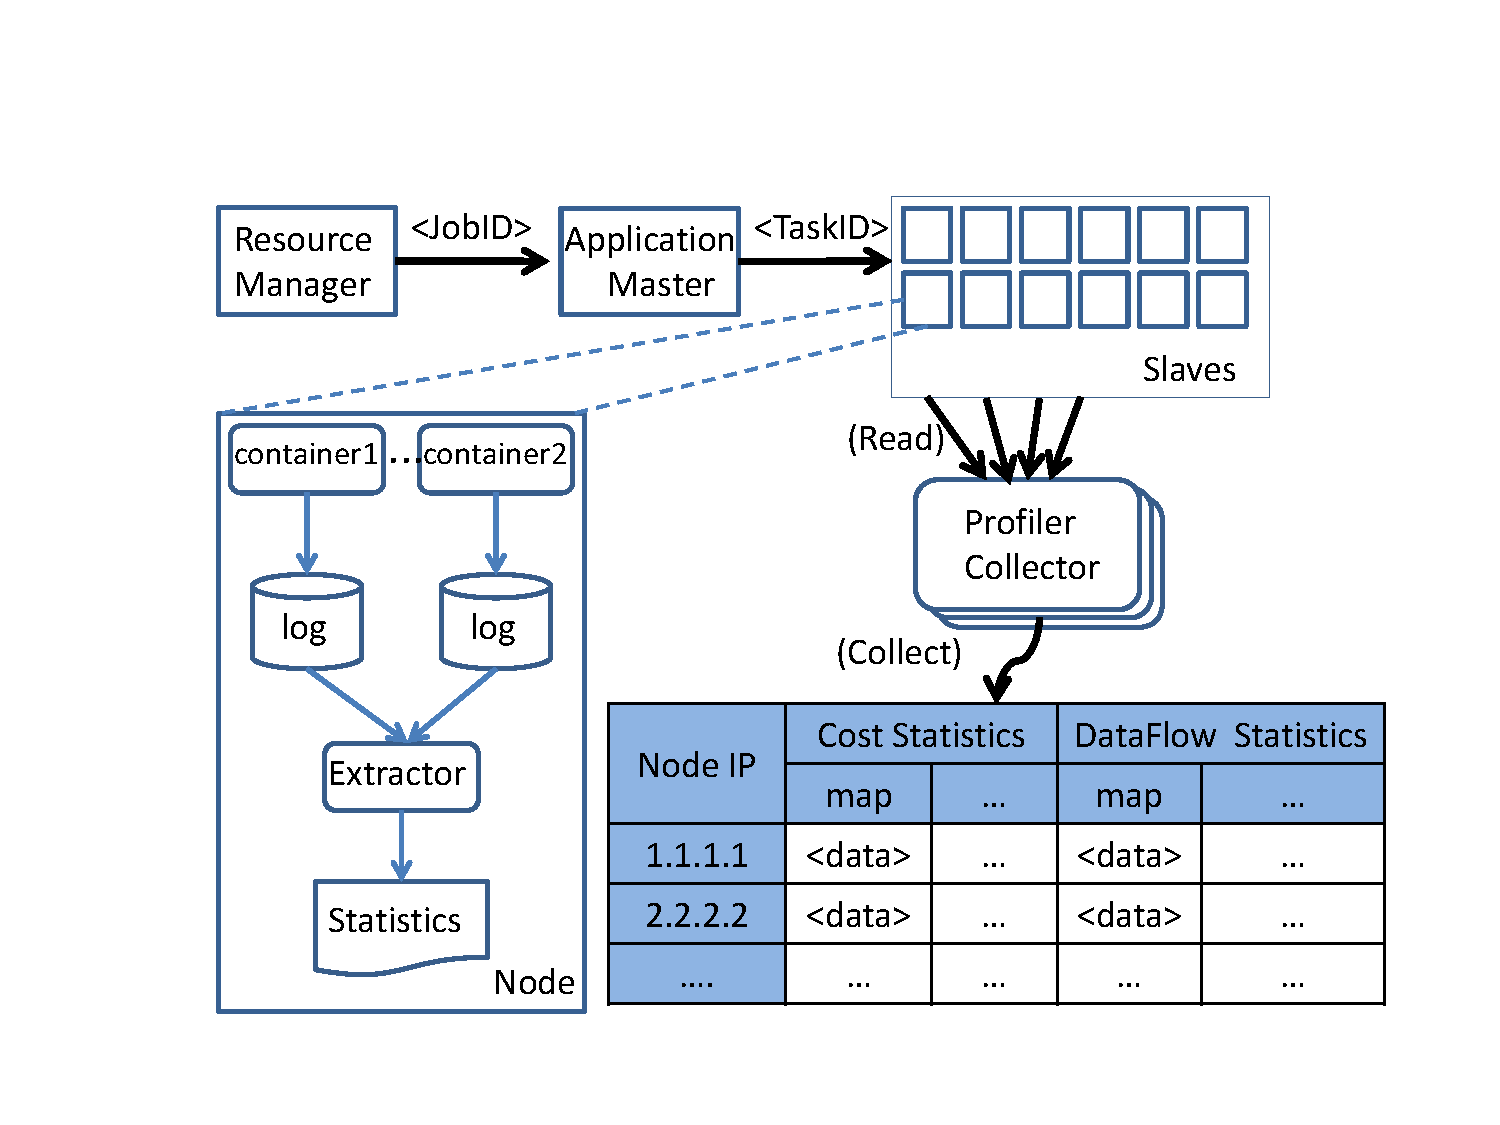
\includegraphics[height=5.5cm, width=8cm]{profiler}
\caption{The Data Flow of LTrace}
\end{center}
\end{figure}

The data flow diagram of the profiler is shown as the figure 2. In order to be a lightweight tools, the LTrace is divided into two separate parts, and these two parts are respectively designed to generate the raw data of data flow and cost when the map and reduce tasks are executing and to off-line extract the execution statistics of the MapReduce job from the raw data. The raw data of the data flow and cost is generated by means of the log system, a small number of logging statements are inserted to record the row data and printed to the local disk when the task is running. Then the log data is extracted to obtain the execution statistics when the execution of the job is complete.

There are multiple MapReduce jobs executed simultaneously on the hadoop cluster and even multiple map and reduce tasks executed simultaneously on the same machine. A MapReduce job consists of multiple map and reduce tasks, and a map or reduce task generates a log file. In order to divide these log files into different partitions that the log files of the same partition are generated by the same MapReduce job, it is essential to add a unique job id to each log. As shown the figure 2, a new MapReduce job is submitted to hadoop cluster, the resource manager allocates the resources for the new jobs  and then start the application master which schedules the execution of the map and reduce tasks for the current MapReduce job. The application master receives a unique job id from the resource manager when it starts, and a unique task id is assigned to the start-up map or reduce task. Therefore, each map or reduce task owns a unique task id, and the task id can also identify the all the tasks scheduled by the same MapReduce job. In summary, this task id if should be automatically added to the logs generated by the task.

Apache Log4j, a popular logging system, is applied in the Apache Hadoop. The Log4j provides a convenient feature: the Mapped Diagnostic Context(MDC), and this context can be used to store values that can be displayed in every log. When the process which executes the map or reduce task is started, the task id should be injected to the MDC, and all the threads and child threads can get the task id from the MDC. In order to automatically add the task id to every log, instead of manually adding the task id to each logging statement, a new layout is implemented to redefine the format of the output logs as follows: $<date, thread, taskId, message>$.

As shown in the figure 2, the Extractor, a component of the LTrace, is deployed on all the machines in the cluster, and it off-line extract the execution statistics from the raw log files. The Profiler Collector, another component of the LTrace, is deployed on the one of the machines in the cluster. This collector collects all the execution statistics extracted by the Extractor from the other machines and stores the statistics into the disk files as shown in figure 2.


\section{An Accurate Performance Model}
This section introduces a new performance model constructed to accurately predict the execution time of the MapReduce job in the Hadoop cluster.

To construct an accurate performance model, there are some effective methods and principles as follows:
\begin{itemize}
\item To accurately predict the execution time of the MapReduce job, this performance model should be able to forecast each execution phase's cost of the job accurately.
\item The output of each execution phase is the input of the next execution phase, hence this model also needs to forecast the volume of each phase's output beside the execution cost.
\item The execution time of the map and reduce task is not the sum of each phase's cost, due to the presence of parallel that multiple phases execute simultaneously. In order to construct an accurate model, it's necessary to confirm whether the parallel exists between multiple phases, and to predict the overlap time between these phases executed in parallel.
\end{itemize}

The execution of a MapReduce job consists of the map and reduce tasks, hence the construction of the performance model is divide two sections as follows.

\subsection{The Cost Model For Map Task}
The execution of the map task, which is described in the section 2, consists of the following phases: read, map, spill and merge. The key of our work is to predict the actual cost of map and spill.

\noindent\textbf{Map and Spill. }The user-defined map function is executed by the main thread to process the input data, and the spill of the buffer data is performed by the spill thread to sort, combine and write the buffer data sequentially.

\noindent\textbf{(i) Execution Procedure}
\begin{figure}[htbp]
\centering
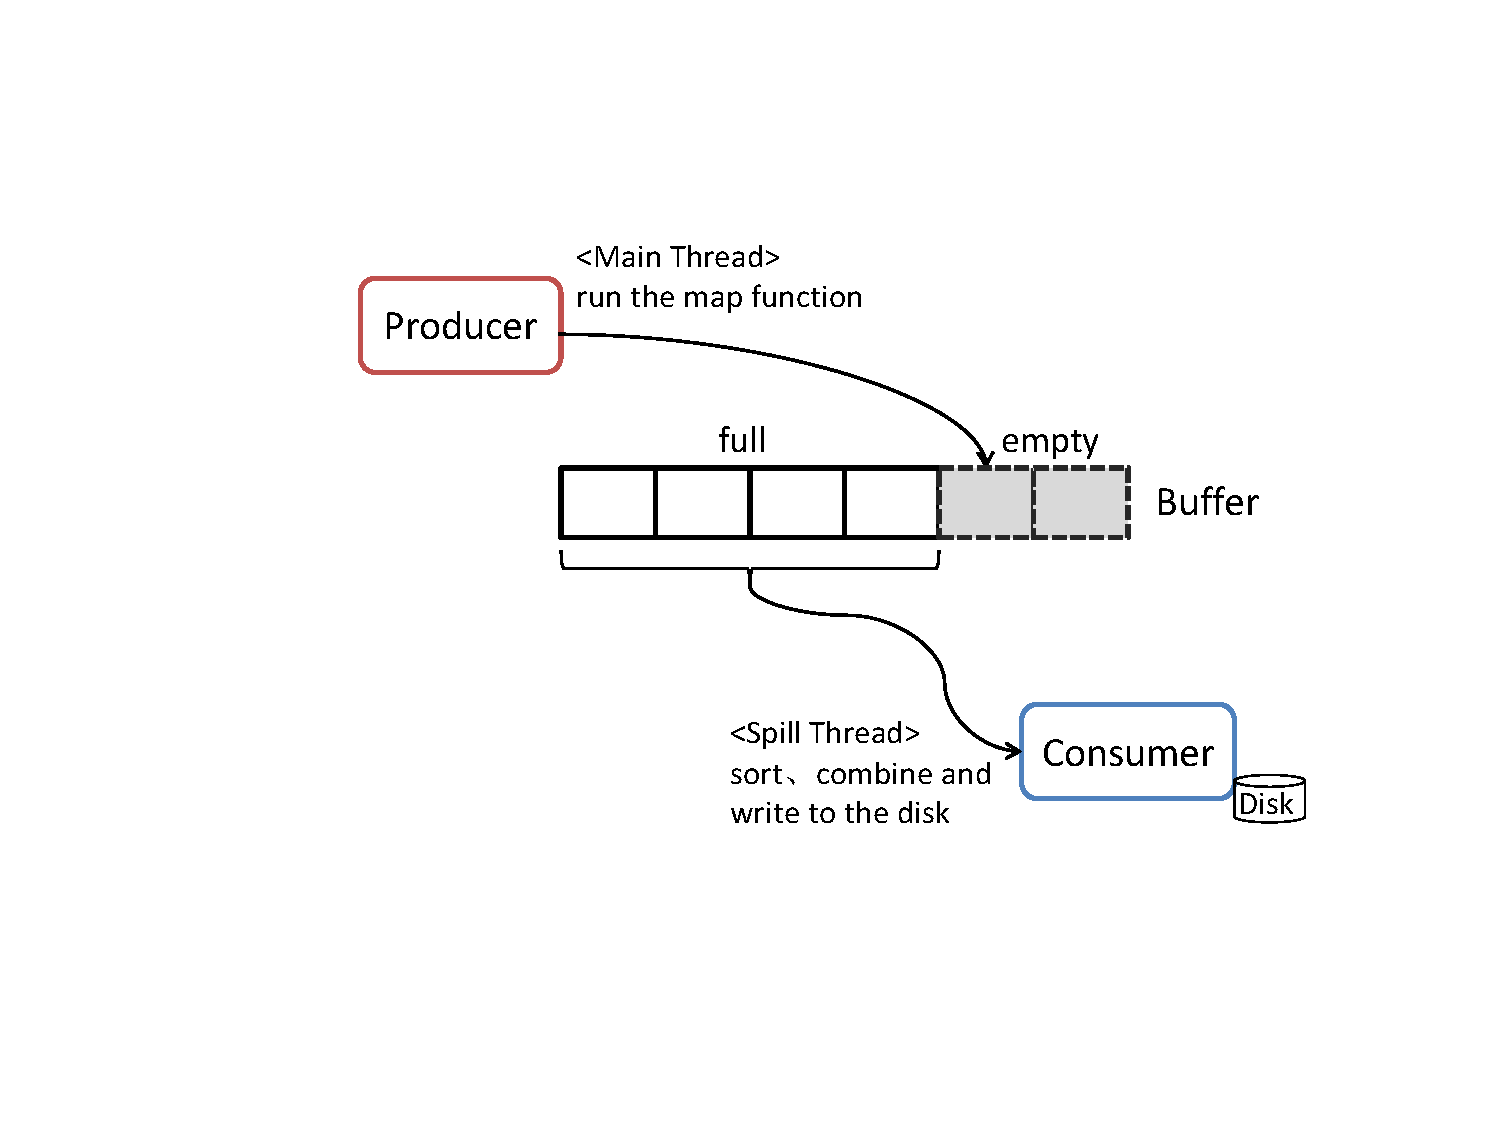
\includegraphics[height=4.5cm, width=8cm]{mapandspill}
\caption{The Interaction between Map and Spill}
\end{figure}

As shown in figure 3, when the main thread executes the map function, the output of the map function is written into the memory buffer. The spill thread starts to spill the outputs cached in the buffer to the disk file when the used space of the buffer reaches the threshold determined by the related configuration parameter. The main thread continues to execute the map function, when the spill thread spills the data into the disk file. The main thread starts to sleep when the buffer is full and stop sleeping after the data in the buffer is written to disk file.

\noindent\textbf{(ii) The Analysis of Key Effect Factors}
\begin{itemize}
\item  \textbf{The cost of map function's execution every time} $m_{cs}$, and \textbf{the number of map function's execution} $mn_d$. The factor $m_{cs}$ is determined by not only the complexity of the user-defined map function but also the execution environment which consists of the resource consumed by map task and the number of executing threads in the map task.
\item  \textbf{The size of memory buffer} $mb_p$, and \textbf{the threshold at which the spill is triggered} $st_p$. These two factors determine when to spill.
\end{itemize}

The total execution time of map and spill is not their linear additivity, due to the parallel execution between map and spill. To predict the total cost of these two phases, we need to estimate not only the individual cost of map and spill, but also their overlap time during which these two phases execute simultaneously. The cost of map is determined by the $m_{cs}$ and $mn_d$, and the cost of spill is determined by the cost of one spill $os_c$ and the number of spill affected by the $mb_p$ and $st_p$. If the $mb_p$ and $st_p$ increase, the $os_c$ increases but the number of spill decreases, therefore it's uncertain whether the cost of spill increases or not. Their overlap time is determined by the $os_c$ and the cost of map when spilling $mws_c$ which is also affected by the $mb_p$ and $st_p$. when the $mb_p$ is fixed, if the $st_p$ increases, the $os_c$ increases but the $mws_c$ might decreases or increases(it's determined by whether the main thread is sleep or not), therefore it's also uncertain whether the overlap time increases or not. In summary, it's challenging to estimate the total execution time of map and spill which is nonlinearly affected by these key factors. We construct the following model to predict the total execution time of map and spill.


\noindent\textbf{(iii) The Construction of Model}

We propose a model to predict the total execution time of map and spill as follows. We need to predict the dataflow of these two phases before estimating the cost.

\emph{DATAFlOW}: The dataflow of these two phases consists of the input and output of each phase. We estimate the output of each phase through the output of last phase and the dataflow statistics captured by the LTrace, for example, the output of map is estimated as follows.
\begin{small}
$$mor_d=mn_d\times\frac{\sum_{i=1}^nmrs_{ds}^i}{n}$$
\end{small}
\emph{where the $mor_d$ is the total number of output records generated by the map function, the $mn_d$ is the number of input records to be processed by the map function, and the $mrs_{ds}^i$ is the records selectivity of the map function performed on the $i$th machine. }
\begin{small}
$$mob_d=mib_d\times\frac{\sum_{i=1}^nmbs_{ds}^i}{n}$$
\end{small}
\emph{where the $mob_d$ is the total size of output bytes generated by the map function, the $mib_d$ is the size of input bytes to be processed by the map function, and the $mbs_{ds}^i$ is the sizes selectivity of the map function performed on the $i$th machine. }
\begin{small}
$$morw_d=\frac{mob_d}{mor_d}$$
\end{small}
\emph{where the $morw_d$ is the average size of each output record generated by the map function.}

Similarly, we estimate the input and output of the spill which consist of the number of records per spill $rps_d$, the number of output records per spill $sor_d$, the size of output bytes per spill $sob_d$, and the number of spills $ns_d$.

\emph{COST}: To predict the total execution time of these two phases, we have to estimate the costs of these two phases and their overlap time as follows.
\begin{small}
\begin{equation}
\begin{split}
mas_c=s_c+ls_c+m_c-otms_c
\end{split}
\end{equation}
\end{small}
\emph{where the $mas_c$ is the total execution time of these two phases, the $s_c$ is the cost of all the spills except the last, the $ls_c$ is the cost of last spill executed by the main thread, the $m_c$ is the cost of the map, and the $otms_c$ is the overlap time between these two phases.}

To predict the total execution time $mas_c$, it's essential to accurately predict the $s_c$, $ls_c$, $m_c$ and the $otms_c$.

The $cSpillCost$ is estimated as follows.
\begin{small}
\begin{equation}
\begin{split}
s_c=ns_d\times os_c
\end{split}
\end{equation}
\end{small}
\emph{where the $ns_d$ is the number of spills executed by the spill thread, and the execution cost per spill $os_c$ which is estimated as follows.}
\begin{small}
\begin{equation}
\begin{split}
os_c=rps_d\times\frac{\sum_{i=1}^ns_{cs}^i}{n}+rps_d\times\frac{\sum_{i=1}^nc_{cs}^i}{n}+sob_d\times \frac{\sum_{i=1}^nw_{cs}^i}{n}\nonumber
\end{split}
\end{equation}
\end{small}
\emph{where the $rps_d$, $rps_d$ and $sob_d$ are estimated by the means introduced above, and the $s_{cs}^i$, $c_{cs}^i$ and the $w_{cs}^i$ are respectively the cost statistics about sorting, combining and writing}

The cost of last spill $ls_c$ is estimated as follows.
\begin{small}
\begin{equation}
\begin{split}
ls_c=(mor_d-ns_d\times rps_d)\times \frac{\sum_{i=1}^ns_{cs}^i}{n}+(mor_d\\
-ns_d\times rps_d)\times \frac{\sum_{i=1}^nc_{cs}^i}{n}+morw_d\times  (mor_d\\
-ns_d\times rps_d)\times \frac{\sum_{i=1}^ncb_{ds}^i}{n}\times \frac{\sum_{i=1}^nw_{cs}^i}{n}
\end{split}
\end{equation}
\end{small}
\emph{where the $ls_c$ is composed of the costs of sorting, combining and writing the buffer data into a new disk file, and the $cb_{ds}^i$ is the data statistics about combining. }

Through the above analysis of the key effect factors, the cost of map function's execution every time is effected by the number of executing threads in the map task. The main thread may execute the map function when the spill thread is spilling the data cached in the buffer into a new file, and the execution speed of the map function is slower due to the simultaneous execution of the spill thread. Therefore, the execution cost of map is divided into two parts as follows.
\begin{small}
\begin{equation}
\begin{split}
m_c=mws_c+mns_c
\end{split}
\end{equation}
\end{small}
\emph{where the $m_c$ is the total execution time of map, the $mws$ is the execution time of map when the spill thread is running and the $mns_c$ is the execution time of map when the spill thread is stopping.}

The spill thread spills the data cached in the buffer in parallel with the main thread which executes the map function, due to the remaining space of the buffer. The main thread starts to sleep when the buffer is full, and the main thread restarts to execute the map function when the spill is completed. Therefore, the estimation of the $mws_c$ and $mns_c$ is complicated, which is closely associated with the remaining space of the buffer.

We assume that there are not enough remaining space in the buffer to hold the output of the map function when the spill thread is executing, and the execution time of the main thread when the spill thread is working is less than the cost of one spill due to the sleep of the main thread. This assumption is judged as follows.
\begin{small}
\begin{equation}
\begin{split}
isMainThrSleep=mwos_c<os_c \nonumber
\end{split}
\end{equation}
\end{small}
\emph{where the $mwos_c$ is the cost of the map when the spill thread is executing, and it is estimated as follows,}
\begin{small}
\begin{equation}
\begin{split}
mwos_c=\frac{mb_p\times (1-st_p)}{(morw_d+16)} \times\frac{\sum_{i=1}^nmws_{cs}^i}{\sum_{i=1}^nmrs_{ds}^i} \nonumber
\end{split}
\end{equation}
\end{small}
\emph{where the $mws_{cs}^i$ is the cost of map function's execution every time when the spill thread is running on the $i$th machine, and it is captured by the LTrace.}

When the above assumption is tenable, the main thread starts to sleep when the buffer is full, and the $mws_c$ and $mns_c$ are estimated as follows.
\begin{small}
\begin{equation}
\begin{split}
mws_c=mwos_c\times (ns_d-1)+Min(\frac{mb_p\times (1-st_p)}{(morw_d+16)} ,mor_d\\
-rps_d\times ns_d)\times \frac{\sum_{i=1}^nmws_{cs}^i}{\sum_{i=1}^nmrs_{ds}^i} \nonumber
\end{split} 
\end{equation}
\end{small}
\begin{small}
\begin{equation}
\begin{split}
mns_c=(mor_d-(ns_d-1 )\times\frac{mb_p\times (1-st_p)}{(morw_d+16)}-Min(mor_d\\
 - rps_d\times ns_d, \frac{mb_p}{(morw_d+16)} 
\times (1-st_p)))\times \frac{\sum_{i=1}^nm_{cs}^i}{\sum_{i=1}^nmrs_{ds}^i} \nonumber
\end{split}
\end{equation}
\end{small}
\emph{where the $m_{cs}^i$ is the cost of map function's execution every time when the spill thread is not running on the $i$th machine, and it is captured by the LTrace.}

When the above assumption is not tenable, the main thread does not sleep due to the enough space of the buffer. The $mws_c$ and $mns_c$ are estimated as follows.
\begin{small}
\begin{equation}
\begin{split}
mws_c=nmws_d \times\frac{\sum_{i=1}^nmws_{cs}^i}{n} \nonumber
\end{split}
\end{equation}
\end{small}
\begin{small}	
\begin{equation}
\begin{split}
mns_c=nmns_d\times \frac{\sum_{i=1}^n m_{cs}^i}{n} \nonumber
\end{split}
\end{equation}
\end{small}
\emph{where the $nmws_d$ is the number of map function's execution when the spill thread is running, and the $nmns_d$ is the number of map function's execution when the spill thread is sleeping, and they are estimated as follows.}
\begin{small}
\begin{equation}
\begin{split}
nmws_d=\frac{os_c\times n}{\sum_{i=1}^n mws_{cs}^i} \times 
(ns_d-1)+Min( \frac{os_c\times n}{\sum_{i=1}^n mws_{cs}^i} 
, \\
\frac{(mor_d-ns_d\times rps_d)\times n}{\sum_{i=1}^nmrs_{ds}^i})  \nonumber
\end{split}
\end{equation}
\end{small}
\begin{small}
\begin{equation}
\begin{split}
nmns_d=mn_d-nmws_d \nonumber
\end{split}
\end{equation}
\end{small}
At last, the $otms_c$ is estimated as follows.
\begin{small}
\begin{equation}
\begin{split}
otms_c=mws_c
\end{split}
\end{equation}
\end{small}
\subsection{The Cost Model For Reduce Task}
The execution of the map task, which is described in the section 2, consists of the following phases: shuffle, merge, reduce and write. The key of our work is to predict the effective cost of shuffle.

\noindent\textbf{Shuffle.} The reduce task reads the corresponding outputs of all the map tasks from the remote machines in the cluster.

\noindent\textbf{(i) Execution Procedure}
\begin{figure}[htbp]
\centering
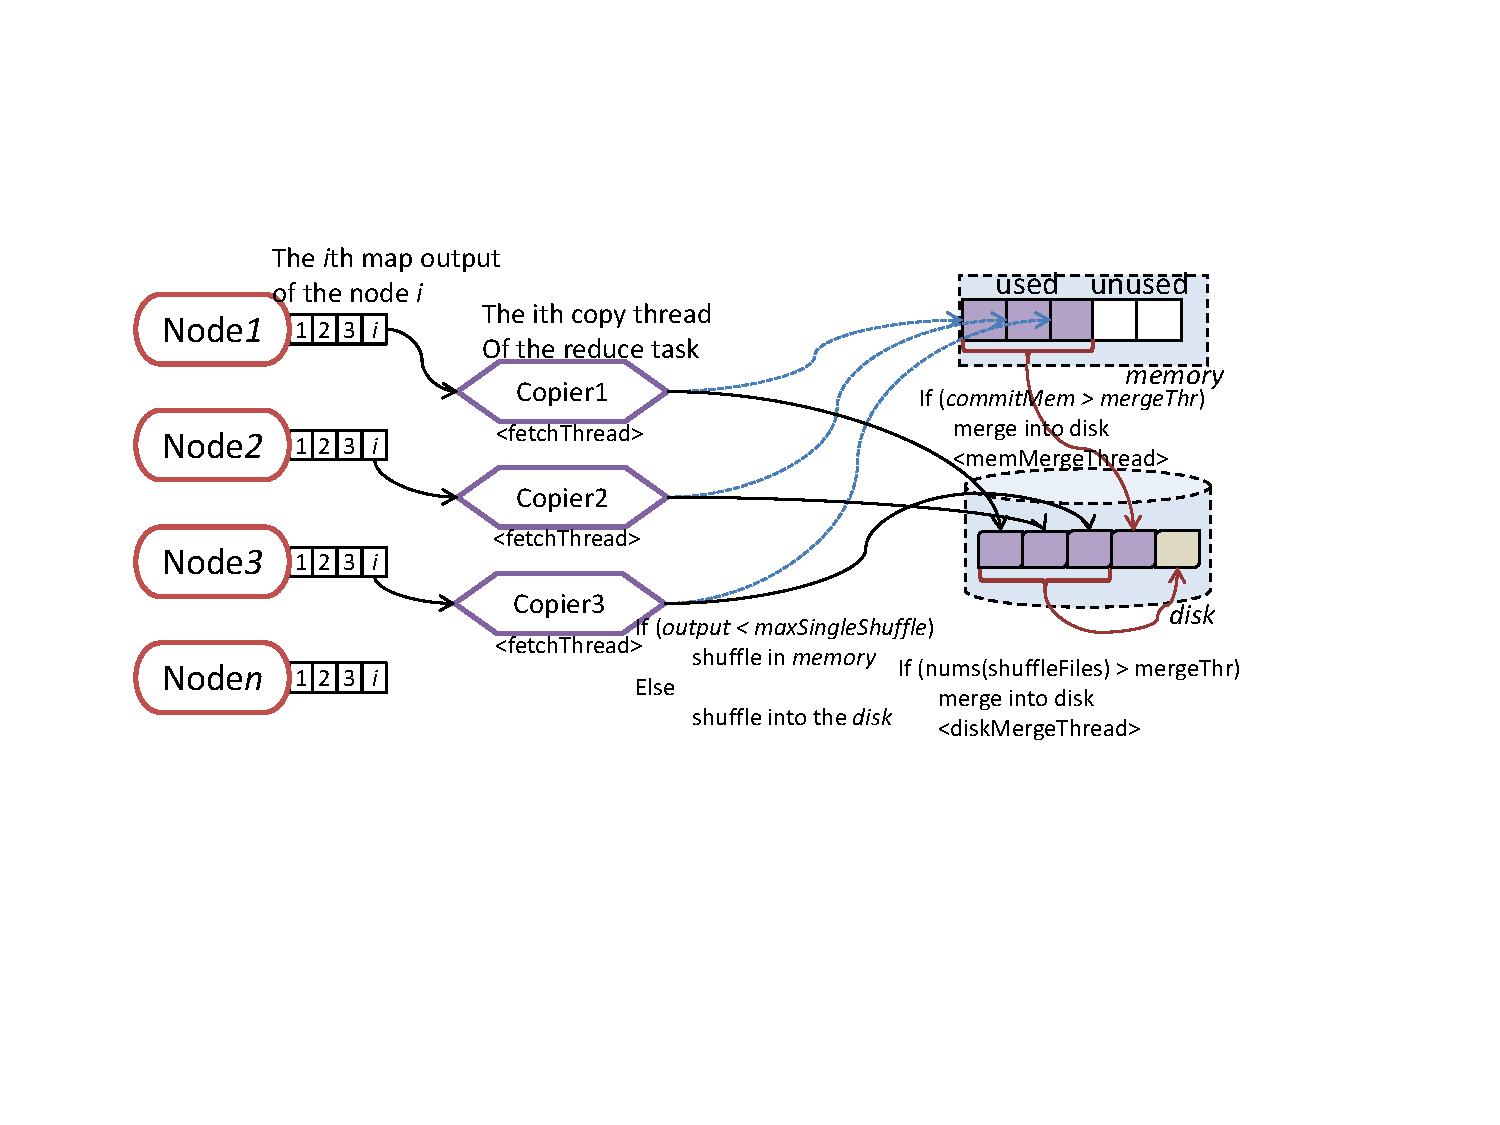
\includegraphics[height=4.5cm, width=9cm]{shuffle}
\caption{The Execution Procedure of Shuffle}
\end{figure}

As shown in figure 4, multiple copy threads of the reduce task are started to simultaneously fetch the corresponding outputs of map tasks from the various machines When there are multiple outputs generated by different map tasks on a machine, only one of these copy threads sequentially fetches these outputs from the target machine.

When the copy thread starts to fetch the output of the completed map task, the output can be written to the memory buffer or a new disk file, which
is determined by the way as shown in figure 4. A merge thread is started, when the used space of the memory buffer or the number of disk files reach the threshold.

\noindent\textbf{(ii) The Analysis of Key Effect Factors}
\begin{itemize}
\item \textbf{The number of the effective copy threads} $nc_p$, the $nc_p$ is the actual number of copy threads which simultaneously fetch the outputs of map tasks from $nc_p$ machines.
\item \textbf{The output of the map task} $mo_d$, and \textbf{the max single shuffle limit} $mssl_p$. These two factors determine whether the map task's output is fetched into the buffer or disk.
\item \textbf{The threshold at which the memory merge is triggered} $mt_p$, and \textbf{the number of disk files at which the disk merge is triggered} $sf_p$. These two factors affect when the merge thread merge the buffer data or the disk files into a new file.
\end{itemize}

\noindent\textbf{(iii) The Construction of Model}

We propose the simulation approach to predict the whole shuffle time of the reduce task. 

\noindent\rule{3.5in}{0.6mm}
\textbf{Algorithm 1} The simulation of shuffling into the buffer
\rule{3.5in}{0.3mm}
\begin{algorithmic}[1]
\Require $mapOutputs$, $numCopies$
\Ensure $cShuffleTime$
\Function{CShMCost}{$mapOutputs, numCopies$}
\State $T_c \gets 0,  T_m \gets 0, T_d \gets 0$
\State $haveShu\gets 0, isM \gets 0, isF \gets 0 $
\State $Outs_m \gets null, Outs_d \gets null $
\State $numOuts_{mtod} \gets 0, copyDests \gets null $
\State $indexDest \gets 0$
\For{$i=0 \to numCopies-1$}
\If{$i<length[mapOutputs]$}
\State $copyDests[i] \gets mapOutputs[i]$
\State $indexDest \gets indexDest + 1$
\Else
\State $copyDests[i] \gets null$
\EndIf
\EndFor
\While{!\Call{IsNull}{$mapOutputs$}}
\For{$t=0 \to numCopies - 1$}
\State $out \gets copyDest[t] $
\If{$out \neq null$ \textbf{and} $T_c >= T_s[out]$}
\State $nums[out] \gets nums[out] - 1$
\State $Outs_m \gets Outs_m + out$
\State $haveShu \gets 1$
\If{\Call{IsMerge}{$MapOuts_m$}}
\State $isM \gets 1$
\State $numOuts_{mtod} \gets size[Outs_m]$
\EndIf
\If{$nums[out] == 0 $}
\State \Call{UpdateCopyDest}{$indexDest,$
        $mapOutputs$}
\EndIf
\If{\Call{IsFull}{$MapOuts_m$}}
\State $isF \gets 1$
\State exit
\EndIf

\EndIf
\EndFor
\If{$havaShu == 1$}
\State $T_c \gets T_c + \Call{ShuCost}{mapOutputs[0]}$
\State $haveShu \gets 0$
\If{$isM == 1$}
\State $T_m \gets \Call{Max}{T_c, T_m}$
\State $T_m \gets T_m + \Call{MemMerge}{$
$MapOuts_m, numOuts_{mtod}, Outs_d}$

\If{$\Call{IsDiskMerge}{Outs_d}$}
\State $T_d \gets \Call{Max}{T_d, T_m}$
\State $T_d \gets \Call{DiskMerge}{Outs_d} + T_d$
\EndIf
\State $isM \gets 0$
\EndIf

\If{$isF == 1$}
\State $\Call{RemoveMemOuts}{Outs_m, $
$numOuts_{mtod}}$
\State $T_c = \Call{Max}{T_c, T_m}$
 \State $isF \gets 0$
\EndIf

\Else
\State $T_{new} \gets \Call{LastedClock}{mapOutputs}$
\State $T_c \gets \Call{Max}{T_c, T_{new}}$
\EndIf

\EndWhile
\State $cShuffleTime \gets \Call{Max}{T_c, T_m, T_d}$
\EndFunction
\end{algorithmic}
\noindent\rule{3.5in}{0.6mm}

In the algorithm 1, the $mapOutputs$ is the set of the map task's outputs on all the machines, each element of this set records the number and the finish time of map tasks simultaneously executing on the one machine. The $T_c$, $T_m$ and $T_d$ respectively are the clock of copy thread, memory merge thread and the disk merge thread, and these clocks record the start or end time of the related trigger event, for example, the $T_m$ records the start and end time of the memory merge executed by the memory merge thread. When a event is trigger by one thread, the start time of the event is updated to be the current clock of that certain thread, and the end time of the event is the sum of this event's cost and the start time. For example, if the buffer data size reach the memory merge threshold after one copy thread fetches the data into the buffer, the memory merge event is trigger, the start time of this memory merge $T_m$ is updated to be the copy thread's clock $T_c$, and then the $T_m$ increases by the cost of this merge thread, which presents the end time of this event. The value of $isM$ indicates whether it's time to start to memory merge thread to merge the buffer data into a new file, and the $isF$ indicates whether the buffer is full. The $Outs_m$ and $Outs_d$ are the outputs of map tasks stored in the memory and disk respectively. The value of $haveShu$ indicates that whether there are map tasks' outputs to be fetched at the moment, if the $haveShu$ is 0, then the $T_c$ needs to be updated as the latest finish time of all the remaining map tasks. The $cShuffleTime$, the cost of shuffle, is the maximum of $T_c$, $T_m$, $T_d$. It is worth to note that our algorithm can predict the effective shuffle time of the reduce task, when there are multiple waves of map tasks and reduce tasks simultaneously running on this cluster.

Similar to the algorithm 1, we can use the similar method to calculate the cost of the shuffle, when the map tasks' outputs are written into the disk.  The $T_c$ and $T_d$ respectively are the clock of copy thread and disk merge thread, and the maximum of the $T_c$ and $T_d$ is the shuffle cost $cShuffleTime$.



\section{Experiment}
In this section, we conduct the following experiments to evaluate the prediction accuracy of the Mr. Prophet, and we compare the effectiveness of this new model with the What-IF~\cite{Herodotou2011Profiling} under a variety of input data and jobs.

\subsection{Experiment Setup}
We deploy a Hadoop cluster as the experimental environment to evaluate the Mr. Prophet. The Hadoop cluster with 16 machines is deployed, one of these machines is deployed as the master which runs the Resource Manager and the NameNode, and the other machines are deployed as the slave which runs the Node Manager and the Data Node.

Each machine in the cluster is with 16$\times$2.40GHz Processors and 50GB memory. The Hadoop version is 2.6.0, and the YARN(Yet Another Resource Negotiator)~\cite{Vavilapalli2013Apache} manages(allocate and deallocate) the resource of the Hadoop cluster. There are totally 240 cpu cores and 480 GB memory in the cluster, each machine in the cluster provides 16 cpu cores and 32 GB memory. Therefore, 240 map or reduce tasks can execute simultaneously, due to a map or reduce task requires 1 cpu core and 2 GB memory by default.

We use the HiBench~\cite{Huang2010The} as the benchmark suit, this benchmark suit contains 13 workloads, and we choose three typical workloads as our experimental workloads which are as follows. Wordcount(which counts the occurrence of each word in the input data.), Terasort(which sorts the input data) and the Pagerank(which is MapReduce implementation of Pagerank algorithm.).

\subsection{The Accuracy of the New Model}
To validate the prediction accuracy of the Mr. Prophet, the MapReduce jobs(Wordcount, Terasort and Pagerank) are required to execute on the Hadoop cluster once, and meanwhile the LTrace extracts the statistics of the MapReduce jobs, which is the prerequisite for the prediction. Then the execution time of these jobs with various input data is predicted by the new model and What-IF respectively as follows.

To illustrate the effectiveness of the new model, we establish the following evaluation indicator.
\begin{small}
\begin{equation}
\begin{split}
I_{accu}=\frac{|T_{wf}-T_a|}{T_a} - \frac{|T_{new}-T_a|}{T_a}
\end{split}
\end{equation}
\end{small}

\emph{where the $I_{acct}$ is the indicator value which represents the improvement of the Mr. Prophet's prediction accuracy relative to the What-IF, the $T_a$ represents the actual execution time of the MapReduce job, the $T_{wf}$ is the execution time predicted by the What-IF, and the $T_{new}$ is the execution time predicted by the Mr. Prophet.}

As shown in the equation (6), the $\frac{|T_{wf}-T_a|}{T_a}$ is the relative error of the What-IF's prediction accuracy, and the $\frac{|T_{new}-T_a|}{T_a}$ is the relative error of the new model's prediction accuracy. The decrease of relative error illustrate that the prediction accuracy of the new model is higher than the What-If's, and the higher the $I_{accu}$, the better the effectiveness of the Mr. Prophet relative to the What-If.

\begin{table}[h]
\caption{The Prediction Accuracy of the MapReduce job's execution time}
\newcommand{\tabincell}[2]{\begin{tabular}{@{}#1@{}}#2\end{tabular}}
\begin{center}
\footnotesize
\begin{tabular}{|c|c|c|c|c|c|}
\hline
\tabincell{c}{\textbf{Job}\\ \textbf{Name}} & \tabincell{c}{\textbf{Input}\\\textbf{(GB)}} & \tabincell{c}{\textbf{Actual}\\\textbf{(sec)}} & \tabincell{c}{\textbf{Mr. Prophet}\\\textbf{(sec)}} & \tabincell{c}{\textbf{What-IF}\\\textbf{(sec)}} & \tabincell{c}{$\textbf{I}_{\textbf{accu}}$\\\textbf{(\%)}}\\
\hline
 wordcount & 2 & 70 & 67 & 75 & 3.0 \\
 \hline
 wordcount & 10 & 123 & 118 &  142 & 11.9 \\
 \hline
 wordcount & 30 & 301 & 292 &  339 & 10.0 \\
 \hline
 wordcount & 50 & 469 & 491 & 541 & 10.6 \\
 \hline
 wordcount & 80 & 742 & 772 & 850 & 10.5 \\
 \hline
 wordcount & 100 & 920 & 960 & 1082 & 13.2 \\
 \hline
 terasort & 30 & 119 & 112 & 132 & 5.0 \\
 \hline
 terasort & 50 & 142 & 130 & 162 & 5.6 \\
 \hline
 terasort & 100 & 305 & 292 & 336 & 5.9 \\
 \hline
 terasort & 200 & 1020 & 960 & 1150 & 6.8 \\
 \hline
 pagerank & 31 & 279 & 266 & 313 & 7.5 \\
 \hline
 pagerank & 51 & 350 & 337 & 385 & 6.5 \\
 \hline
 pagerank & 92 & 645 & 624 & 728 & 9.6 \\
 \hline
\end{tabular}
\end{center}
\end{table}
Table 3 orderly shows the job's actual execution time, the job's execution time respectively predicted by the Mr. Prophet and What-IF, and the $I_{accu}$ which illustrates the enhancement of our Mr. Prophet relative to the What-IF under the various size of input data. As shown in the table 3, all the $I_{accu}$ of various jobs under the different input data  are greater than 0, which illustrates that the prediction accuracy of the Mr. Prophet is better than the What-IF to some extent. For the application Wordcount, when the size of the job's input data reaches the 10 GB, all the $I_{accu}$ are greater than 10\%, which shows that our Mr. Prophet owns much stronger forecasting ability than the What-IF especially for the large input data. This is because when the size of input data is larger, there are more data the reduce task have to process, and then there are more data to shuffle, which is simultaneously processed by the multiple copy threads and merge threads, therefore there are much more overlap time between the copy and merge phases, which can be captured by the Mr. Prophet. For the applications Terasort and Pagerank, all the $I_{accu}$ are less than 10\%, it is because these jobs have over 100 reduce tasks, and the data processed by each reduce task is relatively small amount. Despite all this, the prediction accuracy of our Mr. Prophet is above 94\% for the Terasort and Pagerank. It is noteworthy that all the execution time predicted by the What-IF are greater than the actual execution time, which demonstrates that the executing procedure of Hadoop MapReduce job is extremely complex and it is not simply executed step by step. Therefore, it is necessary to find out the parallels between multiple different phases and quantify the overlap time of these parallel phases.

The execution of MapReduce job consists of the map tasks and reduce tasks, the prediction accuracy of the map and reduce tasks' execution time is shown as the follows.

\begin{table}[h]
\caption{The Prediction Accuracy of the Map Task's execution time }
\newcommand{\tabincell}[2]{\begin{tabular}{@{}#1@{}}#2\end{tabular}}
\begin{center}
\footnotesize
\begin{tabular}{|c|c|c|c|c|c|}
\hline
\tabincell{c}{\textbf{Job}\\\textbf{Name}} & \tabincell{c}{\textbf{Input}\\\textbf{(GB)}} & \tabincell{c}{\textbf{Actual}\\\textbf{(sec)}} & \tabincell{c}{\textbf{Mr. Prophet}\\\textbf{(sec)}} & \tabincell{c}{\textbf{What-IF}\\\textbf{(sec)}} & \tabincell{c}{$\textbf{I}_{\textbf{accu}}$\\\textbf{(\%)}}\\
\hline
 wordcount & 2 & 53.8 & 54.7 & 61.8 & 13.2 \\
 \hline
 wordcount & 10 & 53.1 & 54.7 & 61.8 & 13.4 \\
 \hline
 wordcount & 30 & 52.3 & 54.7 & 61.8 & 13.6 \\
 \hline
 wordcount & 50 & 55.5 & 54.7 & 61.8 & 12.7 \\
 \hline
 wordcount & 80 & 54.4 & 54.7 & 61.8 & 13.1 \\
 \hline
 wordcount & 100 & 53.9 & 54.7 & 61.8 & 13.2 \\
 \hline
 terasort & 30 & 32.6 & 28.4 & 29.2 & N \\
 \hline
 terasort & 50 & 33.5 & 28.4 & 29.2 & N \\
 \hline
 terasort & 100 & 31.2 & 28.4 & 29.2 & N \\
 \hline
 terasort & 200 & 35.9 & 28.4 & 29.2 & N \\
 \hline
 pagerank & 31 & 81.8 & 76.2 & 84.2 & N \\
 \hline
 pagerank & 51 & 80.2 & 76.2 & 84.2 & N \\
 \hline
 pagerank & 92 & 82.4 & 76.2 & 84.2 & N \\
 \hline
\end{tabular}
\end{center}
\end{table}
Table 4 shows the map task's actual execution time, the map task's execution time respectively predicted by the Mr. Prophet and What-IF, and the $I_{accu}$. The input data of the map task has nothing to do with the input data of the MapReduce job, one map task processes a block of the HDFS, and the size of each block is uniform 128 MB by default, which can be specified by the related configuration parameter. Therefore, for the each application, the execution time of all the map tasks predicted by the model is the same due to the same block size of the HDFS. As shown in the table 4, for the application Wordcount, all the $I_{accu}$ are greater than 10\%, and the prediction accuracy of our Mr. Prophet for the map task is above 96\%. However, for the Terasort and Pagerank, our Mr. Prophet can't predict accurately the execution time of the map task, this is because there are extra disk I/O latency during the phase of merge, the map task needs to create a new file and merge the relevant data of all the spill files into this new file for each reduce task, there are over 200 reduce tasks for these two jobs and 16 map tasks running simultaneously on one machine, therefore the disk I/O is so busy ,due to the frequent creation and access to various small files, which increases the latency of the disk I/O request response. Unfortunately, our Mr. Prophet can't capture this latency of disk I/O request response, and the What-IF also doesn't not have this ability. The executing speed of the map task is affected by the number of reduce task to some extent, and it is a valuable experience to tuning the performance of the MapReduce jobs.

\begin{table}[h]
\caption{The Prediction Accuracy of the Reduce Task's execution time }
\newcommand{\tabincell}[2]{\begin{tabular}{@{}#1@{}}#2\end{tabular}}
\begin{center}
\footnotesize
\begin{tabular}{|c|c|c|c|c|c|}
\hline
 \tabincell{c}{\textbf{Job}\\\textbf{Name}} & \tabincell{c}{\textbf{Input}\\\textbf{(GB)}} & \tabincell{c}{\textbf{Actual}\\\textbf{(sec)}} & \tabincell{c}{\textbf{Mr. Prophet}\\\textbf{(sec)}} & \tabincell{c}{\textbf{What-IF}\\\textbf{(sec)}} & \tabincell{c}{$\textbf{I}_{\textbf{accu}}$\\\textbf{(\%)}}\\
\hline
 wordcount & 2 & 13.9 & 12.6 & 12.9 & N \\
 \hline
 wordcount & 10 & 66.5 & 63.5 & 76.6 & 10.7 \\
 \hline
 wordcount & 30 & 245.1 & 239.8 & 277.4 & 11.1 \\
 \hline
 wordcount & 50 & 408.4 & 436.7 & 509.7 & 17.6 \\
 \hline
 wordcount & 80 & 680.3 & 717.4 & 835.2 & 17.3 \\
 \hline
 wordcount & 100 & 863.0 & 905.9 & 1072.2 & 19.7 \\
 \hline
 terasort & 30 & 52.4 & 55.4 & 62.5 & 13.5 \\
 \hline
 terasort & 50 & 69.7 & 72.8 & 86.1 & 19.1 \\
 \hline
 terasort & 100 & 165.7 & 172.4 & 202.1 & 17.9 \\
 \hline
 terasort & 200 & 260.5 & 276.3 & 329.2 & 20.3 \\
 \hline
 pagerank & 31 & 108.2 & 112.1 & 128.2 & 14.8 \\
 \hline
 pagerank & 51 & 175.1 & 184.9 & 208.3 & 13.4 \\
 \hline
 pagerank & 92 & 302.7 & 319.5 & 371.3 & 17.1 \\
 \hline
\end{tabular}
\end{center}
\end{table}
Table 5 shows the reduce task's actual execution time, the reduce task's execution time respectively predicted by the Mr. Prophet and the What-IF, and the $I_{accu}$. The input data of the reduce task has a positive correlation with the MapReduce job's input data when the number of reduce tasks is invariant, there are more map tasks when there are more input data processed by the MapReduce job, therefore there are more output data of all the map tasks to be processed by each reduce task.  As shown in the table 5, for the application Wordcount, our Mr. Prophet doesn't show the stronger ability than the What-IF, when the size of input data is 2 GB, this is because that all the 16 map tasks simultaneously execute on one machine, and the map tasks' outputs to be process by the reduce task are small, therefore there is only one copy thread fetching the map tasks' outputs and not merge thread merging the data in the buffer into the disk. For these three application, when the size of input data is larger, the $I_{accu}$ is higher, which indicates our Mr. Prophet has stronger predictive ability than the What-If, especially when the input data is large. This is because there are more map tasks' outputs to be simultaneously copied into the reduce task by multiple copy threads, and meanwhile the merge threads are started to merge the buffer data or the multiple disk files into the disk file. The overlap time between the copy and merge phases increases rapidly, when the input data is getting larger, therefore it is so necessary to quantify the overlap time, and the unfortunate reality is that the What-IF doesn't have the ability to capture these overlap time. These experiments shows that our Mr. Prophet can make up for the defect of the What-IF.
\begin{figure}[htbp]
\centering
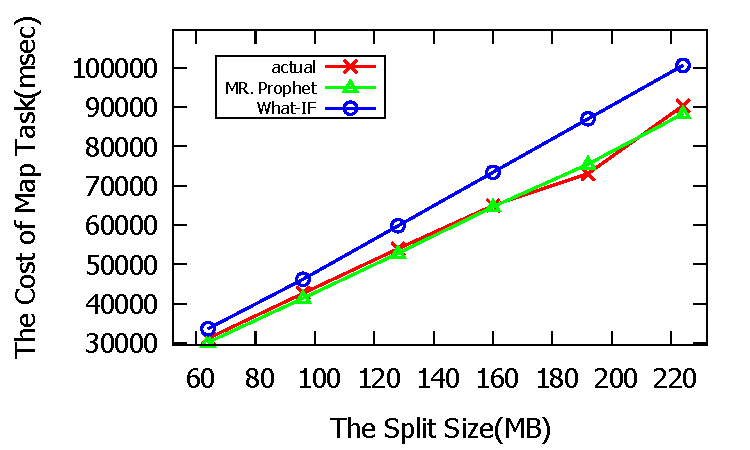
\includegraphics[height=5cm, width=8.5cm]{split}
\caption{The prediction for the map tasks with various split size}
\end{figure}

To more fully illustrate the effectiveness of the Mr. Prophet, we do an extra experiment to compare the prediction accuracy of the Mr. Prophet and What-IF for the map tasks with various input data. We adjust the map task's input size by changing the configuration parameter dfs.block.size, and the parameter value is set from 64 to 224 MB. As shown in the figure 5, our Mr. Prophet owns the strong ability to accurately predict the executing time of the map tasks with various input size. As expected, we can find that all the map tasks' execution time predicted by the What-IF are greater than the actual execution time, and the gap is more and more obvious when the input size increases. This is because the spill thread is started to spill the buffer data into the disk file when the size of buffer data reaches the spill threshold, and the main thread still executes the map function due to the remain free space of the buffer, hence there is overlap time between the map and spill phases. Unfortunately, the What-IF can not capture this overlap time between the map and spill phases. When the input size increases, there are more outputs of the map function to be spilled from the buffer into the disk file, which increases the overlap time accordingly. So what, our Mr. Prophet holds the strong ability to capture these overlap time, which improves the predictive accuracy greatly.


\section{Related Work}
What-IF~\cite{Herodotou2011Profiling} is a performance prediction engine, which is applied to the self-tuning system for the MapReduce called Starfish\cite{Herodotos2011¡°}. The authors propose a model to predict respectively the execution time of the map and reduce task, but it doesn't consider the parallelism between multiple phases inside the map or reduce task. Shi~\cite{Shi2014MRTuner} proposes a novel Producer-Transporter-Consumer(PTC) model, which is adopted by the MRTuner to optimize the configuration parameters of MapReduce jobs. The model address the issues of inter-task parallelization, and this issue occurs when there are reduce and map tasks simultaneously executing. At this moment, the shuffle phase of the reduce task is in parallel with the map task, our Mr. Prophet also holds the ability to predict the effective time of this reduce task's shuffle phase, but the PTC can't capture the multiple phases' overlap time.

There are other researches to predict the MapReduce job's execution time. MRPerf~\cite{Wang2009A} is the existing simulators which predict the execution time of MapReduce job through the simulation. MRPerf provides the fine-grained simulation of the MapReduce job at sub-phase level like our Mr. Prophet. However, the MRPerf has to take a relatively long time to predict the MapReduce job's cost due to the use of external network simulator to predict the cost of data transfers. MRShare~\cite{Nykiel2010MRShare} is a framework to transform a batch of queries into a new batch that will be executed more efficiently, the authors proposes a cost model for this optimization, but this cost model is so simplified and it just considers the total cost of read, sort and write. The related researches\cite{Song2013A}\cite{Lin2012A}\cite{Teng2011SimMapReduce} propose some other approaches to predict the cost of MapReduce jobs, but they don't find the issue of phases parallelism.


\section{Conclusion}
This work presents a performance model of MapReduce Applications with Apache Hadoop, which is useful for making an optimal configuration of Hadoop for improving the application performance.
Different from existing work, we take into account the parallelism between the adjacent processing phases.
With a clear understanding of the MapReduce implementation by reading source code of Hadoop, we give an anatomy of MapReduce job processing. It shows which specific phases a MapReduce job must go through and which adjacent phases are run in parallel for performance consideration.
Then we come up with the performance models for Map and Reduce respectively, where we particularly address the issue of predicting the execution time when two execution phases overlap with each other.
As some parameters in the performance models rely on the characteristics of applications themselves and the specific underlying resources, we design a light-weight instrumentation tool, LTrace, to capture the application and resource specific parameters by running an application with LTrace for only one time.
We have conducted a set of experiments with HiBench workload including WordCount, TeraSort and PageRank jobs. Experimental results with different size of data demonstrate that our model can achieve a prediction accuracy as high as over 94\%, which greatly outperforms the comparing approach.

In future, we will continue to work on how to take advantage of our performance models to generate an optimal configuration for MapReduce applications. Beyond that, though our model works well for the batch jobs, we believe it is worthwhile to consider the commonly used query jobs.  The processing of query jobs depends on the specific query constraints provided by users, which usually involves complex data operations and many map/reduce tasks. This can pose new challenges for the generality of the performance model. Our future work will concern this issue by incorporating other benchmarks such as TPC-DS\cite{Nambiar2006The} and BigBench~\cite{Ghazal2013BigBench}.



% An example of a floating figure using the graphicx package.
% Note that \label must occur AFTER (or within) \caption.
% For figures, \caption should occur after the \includegraphics.
% Note that IEEEtran v1.7 and later has special internal code that
% is designed to preserve the operation of \label within \caption
% even when the captionsoff option is in effect. However, because
% of issues like this, it may be the safest practice to put all your
% \label just after \caption rather than within \caption{}.
%
% Reminder: the "draftcls" or "draftclsnofoot", not "draft", class
% option should be used if it is desired that the figures are to be
% displayed while in draft mode.
%
%\begin{figure}[!t]
%\centering
%\includegraphics[width=2.5in]{myfigure}
% where an .eps filename suffix will be assumed under latex,
% and a .pdf suffix will be assumed for pdflatex; or what has been declared
% via \DeclareGraphicsExtensions.
%\caption{Simulation Results}
%\label{fig_sim}
%\end{figure}

% Note that IEEE typically puts floats only at the top, even when this
% results in a large percentage of a column being occupied by floats.


% An example of a double column floating figure using two subfigures.
% (The subfig.sty package must be loaded for this to work.)
% The subfigure \label commands are set within each subfloat command, the
% \label for the overall figure must come after \caption.
% \hfil must be used as a separator to get equal spacing.
% The subfigure.sty package works much the same way, except \subfigure is
% used instead of \subfloat.
%
%\begin{figure*}[!t]
%\centerline{\subfloat[Case I]\includegraphics[width=2.5in]{subfigcase1}%
%\label{fig_first_case}}
%\hfil
%\subfloat[Case II]{\includegraphics[width=2.5in]{subfigcase2}%
%\label{fig_second_case}}}
%\caption{Simulation results}
%\label{fig_sim}
%\end{figure*}
%
% Note that often IEEE papers with subfigures do not employ subfigure
% captions (using the optional argument to \subfloat), but instead will
% reference/describe all of them (a), (b), etc., within the main caption.


% An example of a floating table. Note that, for IEEE style tables, the
% \caption command should come BEFORE the table. Table text will default to
% \footnotesize as IEEE normally uses this smaller font for tables.
% The \label must come after \caption as always.
%
%\begin{table}[!t]
%% increase table row spacing, adjust to taste
%\renewcommand{\arraystretch}{1.3}
% if using array.sty, it might be a good idea to tweak the value of
% \extrarowheight as needed to properly center the text within the cells
%\caption{An Example of a Table}
%\label{table_example}
%\centering
%% Some packages, such as MDW tools, offer better commands for making tables
%% than the plain LaTeX2e tabular which is used here.
%\begin{tabular}{|c||c|}
%\hline
%One & Two\\
%\hline
%Three & Four\\
%\hline
%\end{tabular}
%\end{table}


% Note that IEEE does not put floats in the very first column - or typically
% anywhere on the first page for that matter. Also, in-text middle ("here")
% positioning is not used. Most IEEE journals/conferences use top floats
% exclusively. Note that, LaTeX2e, unlike IEEE journals/conferences, places
% footnotes above bottom floats. This can be corrected via the \fnbelowfloat
% command of the stfloats package.





% conference papers do not normally have an appendix


% use section* for acknowledgement

% trigger a \newpage just before the given reference
% number - used to balance the columns on the last page
% adjust value as needed - may need to be readjusted if
% the document is modified later
%\IEEEtriggeratref{8}
% The "triggered" command can be changed if desired:
%\IEEEtriggercmd{\enlargethispage{-5in}}

% references section

% can use a bibliography generated by BibTeX as a .bbl file
% BibTeX documentation can be easily obtained at:
% http://www.ctan.org/tex-archive/biblio/bibtex/contrib/doc/
% The IEEEtran BibTeX style support page is at:
% http://www.michaelshell.org/tex/ieeetran/bibtex/
%\bibliographystyle{IEEEtran}
% argument is your BibTeX string definitions and bibliography database(s)
%\bibliography{IEEEabrv,../bib/paper}
%
% <OR> manually copy in the resultant .bbl file
% set second argument of \begin to the number of references
% (used to reserve space for the reference number labels box)
%\begin{thebibliography}{1}
\bibliographystyle{IEEEtran}
\bibliography{biblio}
%\bibitem{IEEEhowto:kopka}
%H.~Kopka and P.~W. Daly, \emph{A Guide to \LaTeX}, 3rd~ed.\hskip 1em plus
%  0.5em minus 0.4em\relax Harlow, England: Addison-Wesley, 1999.

%\end{thebibliography}




% that's all folks
\end{document}


